\chapter{第一格(前)}

\emoji{l_ket} 
《猫的日记》是由"悠闲的xia","大姐姐一样的mifa","稳重的yure","孩子气的feer"四个人登场的欢乐向漫画.

虽然都是Arna的大学的学生,但是由于和日本的学年制度不同,3个人都只有15岁.

今天学校来了一只白猫.

进入了Xia的教室、一边闲逛一边坐上了没有人的桌子.

这是到了休息时间,xia他们跟猫说话的场景。


●1格
\begin{figure}[H]
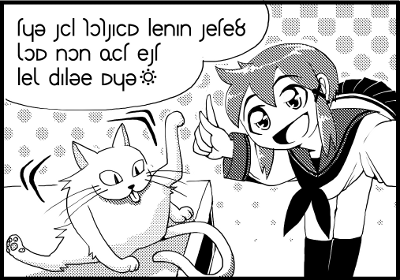
\includegraphics[width=0.5\textwidth]{ARKA/uni1.png}%或者height=\textheight
\end{figure}



\emoji{l_diina} 
这个棕毛就是"悠闲的xia".

她是从首都Arna南边的Kadish搬过来的,那是滨海的都市,是温暖的度假胜地。

Kadish人多是成熟悠闲的类型,xia也是。


\emoji{x_tisse} 
穿着日本的水手服呢.Arbazard也有这样的衣服吗?

看图同时了解文化可是一石二鸟啊.

这样说...哇,没有转写的幻字啊ーヽ(;´·ω·)ノ生幻字啊{\tiny 怕怕}

\footnote{作者注:严格来Arna大学没有制服,为了分辨角色而做了权宜.}

\emoji{l_nakx} 
先从字母转写开始吧.慢慢来.

我也算做了一些转写练习,记得可牢了。

\FiveStar 转写

xia: tyu sil koksaim lenan sete? xom non fit est lex palue myu (xante


\emoji{x_loki} 
嘿,那个数字8一样的东西是问号啊.

最后的文字是啥?工厂的地图记号吗,还是太阳....


\emoji{l_deyu} 
太阳吗?嘟嘟---.这是月亮哦,满月。

表示说话者的语调非常高兴。

满月在Arka叫xante,转写的时候就写"(xante"吧.


\emoji{x_nal} 
話し方を表す文字まであるんだ。面白いね。日本語の(笑)とか♪とかにあたるものかな。
さて、最初の文は"tyu sil koksaim lenan sete?"か。やっぱり本番になると急に単語が難しくなるね。
......あれ?でもtyuとsilは理論編でやったような。tyuは女言葉の「あなた」で、silは未来形を作る副詞だっけ。
あぁ、記憶があいまいだわ(>\_<)。silを辞書で引いてみよ。

----

[名詞]未来、将来
[純副詞]\~{}するだろう。未来時制の副詞。
[動詞]\~{}だろう。未来時制の繋辞。
[形容詞]未来の
[反意語]ses
19:制:sikt(あとで)
【用例】
amir sil 未来のだんな様


----

\emoji{a_niit} 
未来形を作る副詞はsilで合ってるわよ。純副詞のところね。
ほかにも名詞で「未来」って意味があるの。色んな品詞の語義も同時にチェックすると知識が広がるわよ。
さて、"tyu sil koksaim lenan sete?"のsilは何詞の部分を見れば良いでしょうか?


\emoji{x_niit} 
えぇっと......tyuは動詞じゃないから、silが副詞っていう解釈はないわね。
アルカは「主語+動詞+目的語」だから、tyuは主語のはず。となるとsilは動詞だから、この3番目の語義か。
ねぇレイン、未来時制の繋辞って何?いや、未来時制はわかるけどさ。


\emoji{l_rana} 
繋辞はbe動詞のことだよ。
silひとつでwill beになるの。


\emoji{x_lo} 
なるほどね。じゃあ、「あなたは\~{}になるだろう」って言ってるのか。
......何になるんだろ。tyu sil koksaim lenan......。
あ、よく見たらlenanも理論編で出てきたね。%<a href="study_mive1_10.html" 
ってことは、「あなたは私たちのkoksaimになるだろう」ってことね。


\emoji{a_pels} 
さすがにkoksaimは引かないと分からないわね。
参考までに。

\emoji{x_niit} 
同じクラス......あ、クラスメートのことか。
つまり、「あなたは私たちのクラスメートになるだろう」ってことね。


\emoji{a_tia} 
    そのとーり!
    では問題。koksaimのどの部分が「同じ」で、どの部分が「クラス」なのかしら?


\emoji{x_pels} 
えとえと......等式がkoksanで、同じサークルの仲間がkoksemsだから......kokとかkoksとか......。


\emoji{a_niit} 
良い着眼点ね。そう、「同じ」はkokというの。
上下の単語と比べることで、より理解を深めることができるのよ。辞書の良いところよね。


\emoji{x_lo} 
てゆうか、この辞書って物理や地学や気象の用語まで入ってるのね......。
ところで、tyu sil koksaim lenan sete?の最後のseteって何かな。

----

[文末純詞][rente]kok
古

----


\emoji{x_naki} 
あれ、タグだらけ......。
ねぇ、これどういうこと?


\emoji{l_asex_kal} 
これはね、「seteは文末で使う純詞という品詞です」「seteは大人しい女の子が使う言葉です」「意味はkokと同じです」ということを表してるの。
文末純詞は日本語の「\~{}ね」「\~{}さ」「\~{}だよ」「\~{}だわ」「\~{}でしょ?」みたいな単語だよ。
あと、いちど時間があるときに、yunkやmiliaについて調べてみてね。
さて、この場合kokを引くことになるんだけど――

----

[形容詞]同じの
[反意語]koot
[格詞]\~{}と同じく、\~{}と同じで
[文末純詞]\~{}ですね? 確認を求める。
[接続詞]tとkは同じくらい\~{}だ。
[数学]合同
[音楽]シーミレ
13 古:koko。純詞用法は「私の考えと同じか?」という意味から来る。
【成句】
im kok 同時に
【用例】
ti siina miik kok? 君はリンゴが好きだよね?
an kok ti et kai. 私は君くらい大きい。


----

\emoji{x_vesn} 
あ、[文末純詞]はっけん。
へぇ、「\~{}ですね?」という確認を意味するのか。
ということは、"tyu sil koksaim lenan sete?"は「あなたは私たちのクラスメートになるんですね?」という意味か。
あ、そうか。教室に入ってきた猫が住み着いちゃったから、そう言ってるのか。
ふぁー、ようやく分かったよ。


\emoji{l_niit} 
おつかれさま♪


\emoji{x_nal} 
ありがとー。
でもなんか凄い達成感だよ、レイン!
よーし、いったん休憩して、二文目もクリアするぞー!